\subsection{Análisis Exploratorio de Causalidad con DoWhy}

\textbf{Objetivo del Análisis Exploratorio de Causalidad:} Tras identificar las características más influyentes en nuestro modelo a través del análisis SHAP, buscamos entender no solo la correlación, sino también las posibles relaciones causales entre estas características y los resultados de los estudiantes. Utilizando la biblioteca DoWhy, que facilita un enfoque basado en gráficos causales, pretendemos desentrañar las verdaderas relaciones causales detrás de las predicciones de nuestro modelo. Esto nos permitirá diseñar intervenciones más efectivas, basadas no solo en correlaciones observadas, sino en relaciones causales validadas.

\textbf{Metodología Utilizada:} En el ámbito del análisis de causalidad, el primer paso es construir un modelo causal, a menudo representado gráficamente, que captura nuestras creencias iniciales sobre las relaciones causales entre las variables. Este modelo se basa tanto en el conocimiento previo como en la lógica, y establece claramente las variables de tratamiento, resultado y las posibles causas comunes (confundidores). Una vez que tenemos este modelo, podemos identificar el efecto causal de interés y estimarlo utilizando datos observacionales.

Sin embargo, solo basarse en datos observacionales para la estimación causal puede ser engañoso debido a posibles sesgos. Aquí es donde entran los refutadores. Los refutadores en DoWhy son técnicas que nos permiten validar la robustez de nuestros hallazgos causales. Al aplicar diferentes refutadores, como la inserción de una causa común no observada o el uso de un tratamiento placebo, podemos evaluar cuán confiables son nuestras estimaciones causales en presencia de posibles sesgos o supuestos no cumplidos. Si nuestras conclusiones causales se mantienen consistentes incluso después de aplicar estos refutadores, ganamos más confianza en la validez de nuestros hallazgos.

\subsubsection{Análisis de la variable \texttt{hito1}}
Contexto y relevancia específica de la variable \texttt{hito1} dentro de este análisis.
El análisis causal es una herramienta poderosa que nos permite desentrañar las relaciones intrínsecas entre las variables en un conjunto de datos. Tras haber interpretado el modelo con SHAP utilizando un \texttt{RandomForestClassifier}, es imperativo adentrarnos en la causalidad de las variables presentes en nuestro conjunto de datos. Emplearemos la biblioteca \texttt{DoWhy} para discernir y cuantificar el efecto causal de la variable \texttt{hito1} y posteriormente abordaremos las demás variables asociadas a los resultados obtenidos previamente en el Analisis SHAP.

\subsubsection{Modelado del Problema Causal}

El análisis causal se centra en identificar y comprender las relaciones subyacentes entre las variables, en lugar de simplemente observar las correlaciones. Para llevar a cabo un análisis causal efectivo, es crucial establecer un modelo que represente adecuadamente las relaciones causales entre las variables de interés. En este contexto, nos centraremos en la variable \texttt{hito1} como nuestra principal variable de tratamiento.

\begin{lstlisting}[language=Python, caption=Construcción del Modelo Causal para hito1, label=lst:model_causalHito1]
    from dowhy import CausalModel
    # Estableciendo la semilla para el generador de números aleatorios de la biblioteca 'random' en Python.
    # Esto asegura que los números aleatorios generados con la biblioteca 'random' serán reproducibles en cada ejecución.
    random.seed(0)
    np.random.seed(0)
    
    model = CausalModel(
        data=df,
        treatment="hito1",  # Variable tratada (exposición)
        outcome="aprobado",  # Variable de resultado
        graph="""
        digraph {
            e42 -> exitosos;
            e42 -> fallidos;
            e42 -> hito1;
            e29 -> exitosos;
            e29 -> fallidos;
            e29 -> hito1;
            e3 -> exitosos;
            e3 -> fallidos;
            e3 -> hito1;
            e35 -> exitosos;
            e35 -> fallidos;
            e35 -> hito1;
            e18 -> exitosos;
            e18 -> fallidos;
            e18 -> hito1;
            hito1 -> aprobado;
            exitosos -> aprobado;
            fallidos -> exitosos;
            exitosos -> hito1;
        }
        """,
    )
\end{lstlisting}


\begin{figure}[H]
        \centering
        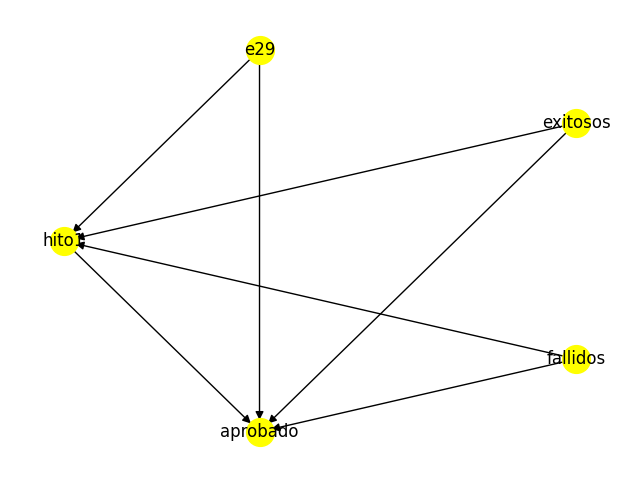
\includegraphics[width=0.9\textwidth]{img/causalidad/graph_causal_model_hito1.png}
        \caption{Representación Gráfica del Modelo Causal}
        \label{fig:modelo_causal_hito1}

\end{figure}

En el código presentado en la Figura \ref{lst:model_causalHito1}, utilizamos la biblioteca \texttt{DoWhy} para construir un modelo causal. La variable de tratamiento es \texttt{hito1}, y la variable de resultado es \texttt{aprobado}. 

La Figura \ref{fig:modelo_causal_hito1} proporciona una visualización gráfica del \texttt{Diagrama Causal Propuesto} en la Figura  [\ref{fig:diagrama_causal_propuesto}] de la subsection \ref{subsec:analisisCausalDowhy}. Esta representación gráfica es esencial porque ofrece una perspectiva visual de cómo se espera que las variables interactúen entre sí. Las flechas indican la dirección de la causalidad, ayudando a entender las posibles rutas a través de las cuales una variable puede influir en otra.

Es importante destacar que este modelo es una representación hipotética de las relaciones causales basada en el conocimiento previo y la comprensión del dominio. La validación y refinamiento del modelo son esenciales para garantizar que las inferencias causales derivadas sean precisas y significativas.

En resumen, el modelado causal es una herramienta poderosa que va más allá de las simples correlaciones y busca entender las verdaderas relaciones subyacentes entre las variables. Al centrarnos en \texttt{hito1}, esperamos descubrir cómo esta variable específica influye en el resultado \texttt{aprobado}, teniendo en cuenta las posibles confusas representadas por las causas comunes.


\subsubsection{Identificación y Estimación del Efecto Causal}

Una vez establecido el modelo causal, el siguiente paso es identificar y cuantificar el efecto causal de la variable \texttt{hito1} sobre \texttt{aprobado}. Esta fase del análisis proporciona una medida cuantitativa del impacto directo de \texttt{hito1} en la probabilidad de aprobación.

\begin{figure}[H]
    \centering
    \begin{minipage}{0.5\textwidth}
        \begin{lstlisting}[language=Python, caption=Proceso de Identificación y Estimación del Efecto Causal, label=lst:IdentificarEstimarefectoCausalHito1]
identified_estimand = model.identify_effect(
    proceed_when_unidentifiable=True
)

estimate = model.estimate_effect(
    identified_estimand,
    test_significance=True,
    method_name="backdoor.econml.dml.DML",
    control_value=0,
    treatment_value=1,
    target_units="ate",
    method_params={
        "init_params": {
            "model_y": RandomForestRegressor(random_state=0),
            "model_t": RandomForestRegressor(random_state=0),
            "model_final": RandomForestRegressor(
                max_depth=10,
                min_samples_split=10,
                min_samples_leaf=5,
                random_state=1502,
                n_estimators=500,
            ),
            "featurizer": None,
        },
        "fit_params": {},
    },
)
\end{lstlisting}
    \end{minipage}
    \hfill
    \begin{minipage}{0.45\textwidth}
        \centering        
        \begin{tabular}{lp{0.6\linewidth}}
            \toprule
            \textbf{Resultado} & \textbf{Valor} \\
            \midrule
            Valor Medio & -0.20362315317793425 \\
            P-Value & 0.111 \\
            \bottomrule
        \end{tabular}
        \caption{Resultados de la Estimación del Efecto Causal para \texttt{hito1}}
        \label{tab:efecto_causal_hito1}
    \end{minipage}
\end{figure}

El código utiliza la biblioteca \texttt{DoWhy} para identificar y estimar el efecto causal con el método \texttt{backdoor.econml.dml.DML}, basándose en investigaciones previas que respaldan el uso del modelo \texttt{RandomForestRegressor} para este análisis, como se discutió en la subsección \texttt{Comparación de algoritmos} \ref{subsec:comparaAlgoritmos}.

El \say{Valor Medio} en la Tabla \ref{tab:efecto_causal_hito1} indica que, en promedio, un incremento unitario en \texttt{hito1} disminuye la probabilidad de aprobar en un \(20.36\% \).

\paragraph{Explicación de los Resultados y Fórmulas:}

\begin{enumerate}
    \item \textbf{Estimand Identificado}:
    \begin{itemize}
        \item \textbf{Tipo}: \texttt{EstimandType.NONPARAMETRIC\_ATE} - Indica que el estimand es no paramétrico para el Efecto de Tratamiento Promedio (ATE).
        \item \textbf{Expresión}:
        \[
        \frac{d}{d\texttt{hito1}}E[\texttt{aprobado}|\texttt{exitosos}]
        \]
        Esta expresión representa la derivada de la expectativa de \texttt{aprobado} respecto a \texttt{hito1}, manteniendo constante \texttt{exitosos}.
        
        \item \textbf{Suposición}:
        \begin{align}
            \text{Si } U &\rightarrow \texttt{hito1} \text{ y } U \rightarrow \texttt{aprobado} \text{ entonces } \nonumber \\
            P(&\texttt{aprobado}|\texttt{hito1},\texttt{exitosos},U) = P(\texttt{aprobado}|\texttt{hito1},\texttt{exitosos})
        \end{align}
        Esta suposición, llamada de falta de confusión, establece que cualquier variable no observada \( U \) que afecte tanto a \texttt{hito1} como a \texttt{aprobado} no cambia la distribución condicional de \texttt{aprobado}.
    \end{itemize}
    
    \item \textbf{Estimand Realizado}:
    \[ 
    \texttt{aprobado} \sim \texttt{hito1} + \texttt{exitosos}
    \]
    Representa una regresión lineal de \texttt{aprobado} en función de \texttt{hito1} y \texttt{exitosos}.
    
    \item \textbf{Estimación}:
    \begin{itemize}
        \item \textbf{Valor Medio}: \( -0.20362315317793425 \) - Efecto promedio estimado de \texttt{hito1} sobre \texttt{aprobado}.
        \item \textbf{P-Value}: \( 0.111 \) - Medida de la significancia estadística de la estimación.
    \end{itemize}
\end{enumerate}

\paragraph{Resumen:}
Se identificó y cuantificó el efecto causal de \texttt{hito1} sobre \texttt{aprobado} usando el método \texttt{backdoor.econml.dml.DML} de la biblioteca \texttt{DoWhy}. La expresión del estimand y la suposición de falta de confusión permiten una comprensión matemática del modelo causal. La estimación reveló un efecto negativo de \texttt{hito1} sobre \texttt{aprobado}, aunque no es estadísticamente significativo al nivel del \(5\%\) dado el valor de \( p = 0.111 \). 


\subsubsection{Refutador de Datos Aleatorios}

El análisis causal no solo se centra en identificar y estimar efectos causales, sino también en validar la robustez de estas estimaciones. Una herramienta clave en esta validación es el refutador de datos aleatorios. Su propósito es evaluar la sensibilidad de nuestro estimado ante la introducción de una causa común aleatoria, lo que nos ayuda a discernir si el estimado es genuino o si podría ser influenciado por variables no observadas.

\begin{minipage}{0.5\textwidth}
    \begin{lstlisting}[language=Python, caption=Refutador de datos aleatorios para \texttt{hito1}, label=lst:RefutadorDatosAleatoriosHito1]
refute1 = model.refute_estimate(
     identified_estimand, estimate, 
     method_name="random_common_cause"
)
\end{lstlisting}
\end{minipage}
\hfill
\begin{minipage}{0.45\textwidth}
    \begin{table}[H]
        \centering        
        \begin{tabular}{lp{0.6\linewidth}}
            \toprule
            \textbf{Resultado} & \textbf{Valor} \\
            \midrule
            Estimado Original & -0.20362315317793425 \\
            Nuevo Efecto & -0.11640820377631846 \\
            p-value & 0.56 \\
            \bottomrule
        \end{tabular}
        \caption{Resultados del Refutador de Datos Aleatorios para \texttt{hito1}}
        \label{tab:refutador_datos_aleatorios_hito1}
    \end{table}
\end{minipage}

El código en el Listado \ref{lst:RefutadorDatosAleatoriosHito1} introduce una nueva causa común aleatoria al modelo y recalcula el efecto causal. Los resultados de esta refutación se presentan en la Tabla \ref{tab:refutador_datos_aleatorios_hito1}. Aunque el \say{Nuevo Efecto} (-0.2036) difiere del \say{Estimado Original} (-0.11640), el p-value de 0.56 indica que esta diferencia no es estadísticamente significativa al nivel convencional del 5\%. Esto refuerza la confianza en que nuestro estimado original es robusto y no es altamente susceptible a la influencia de variables no observadas.



\subsubsection{Refutador de Causa Común No Observada}

El análisis causal no solo busca identificar y estimar efectos causales, sino también validar la robustez de estas estimaciones frente a posibles sesgos. El refutador de causa común no observada es una herramienta que nos permite evaluar la sensibilidad de nuestro estimado ante la introducción de una causa común no observada en el modelo.

\begin{minipage}{0.5\textwidth}
    \begin{lstlisting}[language=Python, caption=Refutador de causa común no observada para \texttt{hito1}, label=lst:RefutadorCausaComúnNoObservadaHito1]
refute2 = model.refute_estimate(
    identified_estimand,
    estimate,
    method_name="add_unobserved_common_cause",
    confounders_effect_on_treatment="binary_flip",
    confounders_effect_on_outcome="binary_flip",
    effect_strength_on_treatment=0.01,
    effect_strength_on_outcome=0.02,
)
\end{lstlisting}
\end{minipage}
\hfill
\begin{minipage}{0.45\textwidth}
    \begin{table}[H]
        \centering
        \begin{tabular}{lp{0.6\linewidth}}
            \toprule
            \textbf{Resultado} & \textbf{Valor} \\
            \midrule
            Estimado Original & -0.20362315317793425 \\
            Nuevo Efecto & 0.17265953316553373 \\
            \bottomrule
        \end{tabular}
        \caption{Resultados del Refutador de Causa Común No Observada para \texttt{hito1}}
        \label{tab:refutador_causa_no_observada_hito1}
    \end{table}
\end{minipage}

El código en el Listado \ref{lst:RefutadorCausaComúnNoObservadaHito1} introduce una causa común no observada al modelo y recalcula el efecto causal. Los resultados de esta refutación se presentan en la Tabla \ref{tab:refutador_causa_no_observada_hito1}. La notable diferencia entre el \say{Estimado Original} (-0.2036) y el \say{Nuevo Efecto} (0.17265) indica que nuestro estimado es sensible a la presencia de variables no observadas. Esta sensibilidad subraya la importancia de considerar posibles sesgos en el análisis causal y de interpretar los resultados con precaución.


\subsubsection{Refutador de Tratamiento Placebo}

El análisis causal no solo busca identificar y estimar efectos causales, sino también validar la robustez de estas estimaciones frente a posibles sesgos. El refutador de tratamiento placebo es una herramienta que nos permite evaluar la sensibilidad de nuestro estimado ante la introducción de un tratamiento ficticio, es decir, un tratamiento que no tiene ningún efecto real sobre el resultado.

\begin{minipage}{0.5\textwidth}
    \begin{lstlisting}[language=Python, caption=Refutador de tratamiento placebo para \texttt{hito1}, label=lst:RefutadorTratamientoPlaceboHito1]
refute3 = model.refute_estimate(
    identified_estimand,
    estimate,
    method_name="placebo_treatment_refuter",
    placebo_type="permute",
)
\end{lstlisting}
\end{minipage}
\hfill
\begin{minipage}{0.45\textwidth}
    \begin{table}[H]
        \centering
        \begin{tabular}{lp{0.6\linewidth}}
            \toprule
            \textbf{Resultado} & \textbf{Valor} \\
            \midrule
            Estimado Original & -0.20362315317793425  \\
            Nuevo Efecto & 0.01788451392154416 \\
            p-value & 0.96 \\
            \bottomrule
        \end{tabular}
        \caption{Resultados del Refutador de Tratamiento Placebo para \texttt{hito1}}
        \label{tab:refutador_placebo_hito1}
    \end{table}
\end{minipage}

El código en el Listado \ref{lst:RefutadorTratamientoPlaceboHito1} introduce un tratamiento ficticio y recalcula el efecto causal. Los resultados de esta refutación se presentan en la Tabla \ref{tab:refutador_placebo_hito1}. El \say{Estimado Original} (-0.20362) y el \say{Nuevo Efecto} (0.0178), cercano a cero, y un p-value elevado de 0.96, sugieren que el tratamiento real, \texttt{hito1}, no tiene un efecto significativo sobre el resultado. Esta evidencia indica que los resultados obtenidos inicialmente podrían ser atribuidos al azar y no necesariamente a la influencia real de \texttt{hito1} sobre \texttt{aprobado}.

\paragraph{Resumen:} El análisis causal de \texttt{hito1} se centró en desentrañar las relaciones intrínsecas con la variable \texttt{aprobado}. Se estableció un modelo causal utilizando \texttt{DoWhy}, representando las relaciones causales entre \texttt{hito1} y otras variables relevantes. La Figura \ref{fig:modelo_causal_hito1} proporciona una visualización gráfica de este modelo.

Posteriormente, se identificó y cuantificó el efecto causal de \texttt{hito1} sobre \texttt{aprobado}, revelando un efecto promedio de -0.2036, lo que indica una disminución del 20.36\% en la probabilidad de aprobar con un incremento unitario en \texttt{hito1}.

Se realizaron refutaciones para validar la robustez del estimado. El refutador de datos aleatorios mostró que el estimado es robusto y no es altamente susceptible a la influencia de variables no observadas. Sin embargo, el refutador de causa común no observada sugirió sensibilidad a variables no observadas. Finalmente, el refutador de tratamiento placebo indicó que el tratamiento real, \texttt{hito1}, podría no tener un efecto significativo sobre el resultado.


\subsubsection{Análisis exploratorio iterativo de las variables seleccionadas}
Después de analizar la variable \texttt{hito1}, extendemos nuestro análisis a otras variables de interés identificadas en la predicción SHAP. Para ello, hemos creado un array \texttt{preguntasGuia} que contiene las variables a investigar, y una variable \texttt{outcome\_variable} para representar el resultado de interés, en este caso, \texttt{aprobado}. A continuación, iteramos sobre cada variable en \texttt{preguntasGuia}, aplicando el mismo proceso analítico empleado previamente en \texttt{hito1}. Los resultados de cada iteración se almacenan en una lista llamada \texttt{results} para su posterior análisis y comparación.

\begin{lstlisting}[language=Python, caption=Proceso de análisis iterativo, label=lst:analisisIterativo]
# Array preguntasGuia treatment
preguntasGuia = [
    "hito1",
    "fallidos",
    "exitosos",
    "e42",
    "e35",
    "e29",
    "e18",
    "e3",
]
# Variable outcome
outcome_variable = "aprobado"
# Lista para almacenar los resultados
results = []
# Función para ejecutar el modelo causal
def run_causal_model(treatment_variable, outcome_variable):
    # Paso 1: Modelar un problema causal
    model = CausalModel(
        data=df,
        treatment=treatment_variable,
        outcome=outcome_variable,
        graph="""
            digraph {        
                e42 -> exitosos;
                e42 -> fallidos;
                e42 -> hito1;
                e29 -> exitosos;
                e29 -> fallidos;
                e29 -> hito1;
                e3 -> exitosos;
                e3 -> fallidos;
                e3 -> hito1;
                e35 -> exitosos;
                e35 -> fallidos;
                e35 -> hito1;
                e18 -> exitosos;
                e18 -> fallidos;
                e18 -> hito1;
                hito1 -> aprobado;
                exitosos -> aprobado;
                fallidos -> exitosos;
                exitosos -> hito1;
            }
            """,
    )
    # ... (resto del código es el mismo utilizado en el análisis de hito1)

    print("fin: " + str(treatment_variable))
    # Obtener el valor p del test de significancia
    significance_test_result = estimate.test_stat_significance()
    p_value = significance_test_result["p_value"]
    # Asegurando devolver todos los valores más importantes para posibles análisis a futuro
    return {
        "Variable de Tratamiento": treatment_variable,
        "Variable de Resultado": outcome_variable,
        "Estimación del Efecto Causal": estimate.value,
        "Valor p": p_value,
        "Tipo (Causa Común Aleatoria)": refute1.refutation_type,
        "CCA Efecto Estimado": refute1.estimated_effect,
        "CCA - Nuevo Efecto": refute1.new_effect,
        "CCA - Valor p": refute1.refutation_result["p_value"],
        "Tipo (Causa Común No Observada)": refute2.refutation_type,
        "CCNO - Efecto Estimado": refute2.estimated_effect,
        "CCNO - Nuevo Efecto": refute2.new_effect,
        "Tipo (Tratamiento Placebo)": refute3.refutation_type,
        "TP - Efecto Estimado": refute3.estimated_effect,
        "TP - Nuevo Efecto": refute3.new_effect,
        "TP - Valor p": refute3.refutation_result["p_value"],
    }
# Iterar sobre cada variable en preguntasGuia y el outcome aprobado
for pregunta in preguntasGuia:
    result = run_causal_model(pregunta, outcome_variable)
    results.append(result)
\end{lstlisting}

El grafico causal obtenido por cada hiteracion se mantiene en su forma de explicar la relacion entre \texttt{treatment} y \texttt{outcome}, presentanda en la Figura [\ref{fig:modelo_causal_hito1}].

\subsubsection{Resultados de la Iteración}

Antes de presentar los resultados de la iteración, se explican las abreviaturas utilizadas en la tabla:
\begin{itemize}
    \item CCA: Causa Común Aleatoria.
    \item CCNO: Causa Común No Observada.
    \item TP: Tratamiento Placebo.
\end{itemize}

Los términos \say{Nuevo Efecto} y \say{Valor p} se refieren a los resultados obtenidos en los análisis respectivos.

\begin{table}[H]
    \centering
    \resizebox{\textwidth}{!}{%      
        \begin{tabular}{cccccccccc}
            \hline
            No. & \makecell{Variable de\\ Tratamiento} & \makecell{Estimación del\\ Efecto Causal} & \makecell{Valor p} & \makecell{CCA \\ Nuevo Efecto} & \makecell{CCA \\ Valor p} & \makecell{CCNO \\ Nuevo Efecto} & \makecell{TP \\ Nuevo Efecto} & \makecell{TP \\ Valor p} \\
            \hline
            1 & e42 & 0.224736 & 0.105 & 0.068243 & 0.04 & -0.106769 & 0.025288 & 0.76 \\
            2 & hito1 & -0.203623 & 0.111 & -0.116408 & 0.56 & 0.172660 & 0.017885 & 0.96 \\
            3 & e18 & 0.130773 & 0.276 & -0.045586 & 0.06 & 0.025984 & -0.031051 & 1.00 \\
            4 & fallidos & -0.117432 & 0.288 & 0.009270 & 0.60 & -0.130266 & 0.027725 & 0.78 \\
            5 & e29 & -0.058810 & 0.322 & 0.219796 & 0.04 & 0.047657 & -0.000015 & 1.00 \\
            6 & exitosos & 0.034945 & 0.430 & 0.038086 & 0.98 & 0.391752 & 0.013166 & 0.98 \\
            7 & e3 & -0.027964 & 0.435 & 0.126084 & 0.10 & 0.093429 & 0.019055 & 0.76 \\
            8 & e35 & 0.006278 & 0.494 & 0.042187 & 0.74 & -0.090410 & 0.006603 & 0.92 \\
            \hline
        \end{tabular}
    }
    \caption{Resultados de la iteración con las variables.}
    \label{tab:resultados_iteracion}
\end{table}

A continuación, se presentan los resultados en un grafico para tener una mejor comprencion de los resultados.

\begin{figure}[H]
    \centering
    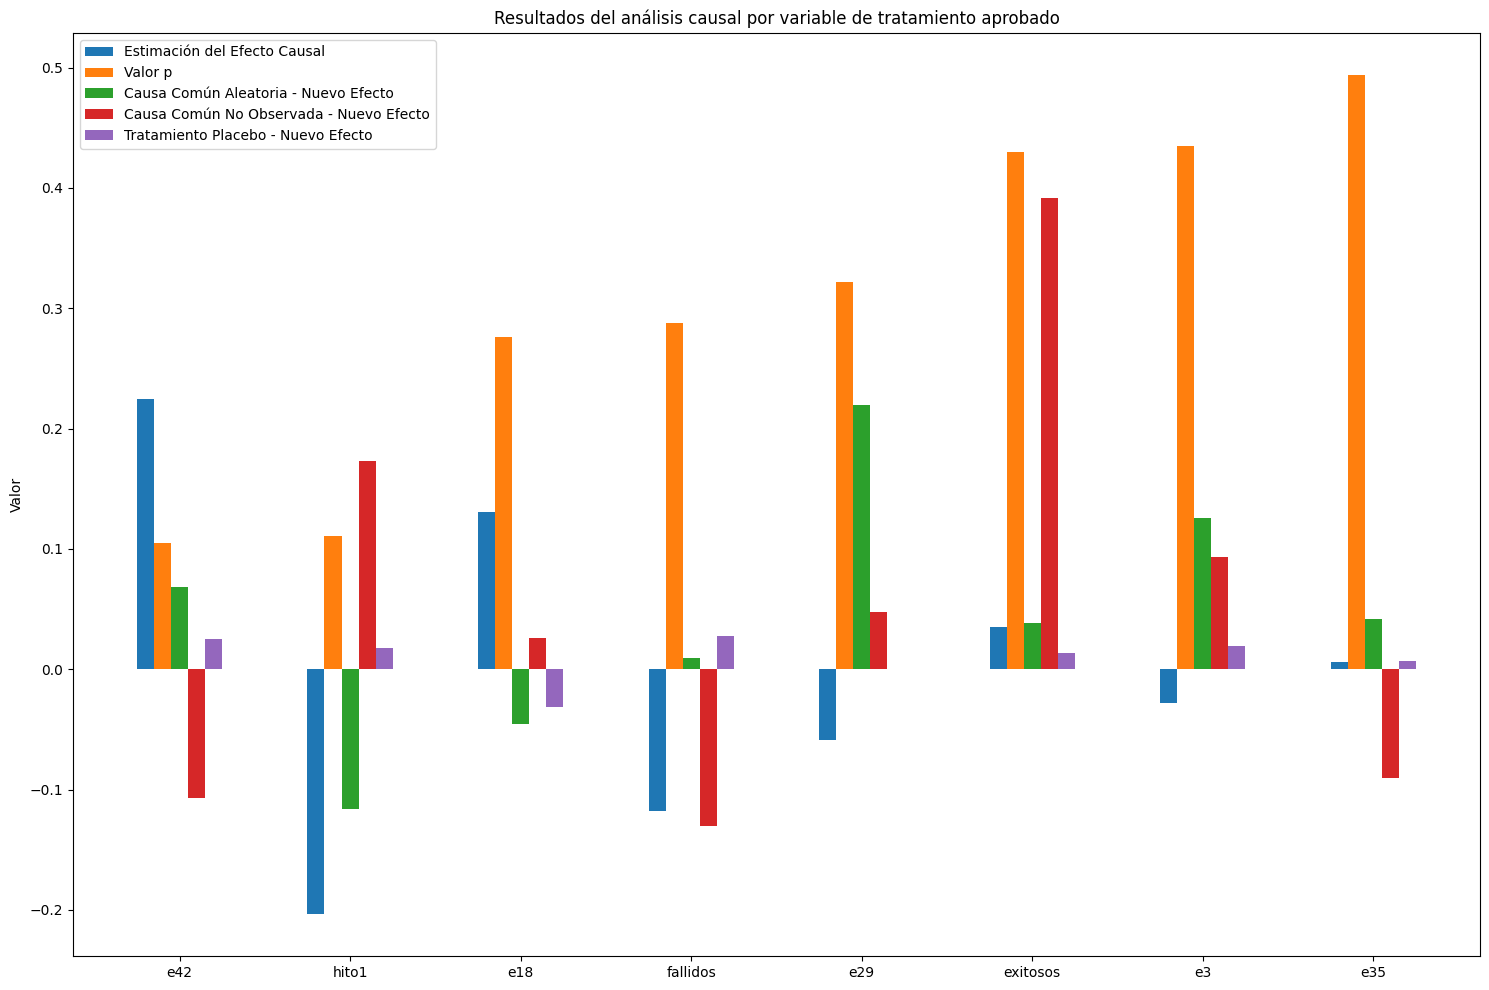
\includegraphics[width=0.8\textwidth]{img/causalidad/grafico_resultados_variables_full.png}
    \caption{Resultados de la iteración con las variables.}
    \label{fig:grafico_iteracion_variables_full_dowhy}
\end{figure}

\textbf{Conclusión}

A partir del análisis causal ejecutado, se exploró cómo diferentes variables asociadas a una guía de apoyo podrían afectar la probabilidad de aprobar la primera evaluación del curso. Las variables examinadas incluyeron \texttt{hito1}, \texttt{exitosos}, \texttt{fallidos}, \texttt{e42}, \texttt{e35}, \texttt{e29}, \texttt{e18} y \texttt{e3}.

\vspace{1em}  % Agrega espacio vertical entre las secciones

\textbf{Resultados Numéricos}

Las estimaciones de los modelos causales y los valores p correspondientes para el tratamiento placebo se presentan a continuación:

\begin{enumerate}
    \item \textbf{Estimación del Efecto Causal}:
        \begin{itemize}
            \item Se identificaron asociaciones entre las variables de interés y la probabilidad de aprobar, aunque la magnitud y dirección de estas asociaciones varían.
        \end{itemize}
    
    \item \textbf{Resultados Numéricos}:
        \begin{itemize}
            \item \textbf{Modelo e42}:
                \begin{itemize}
                    \item Estimación del Efecto Causal: 0.224736
                    \item Valor p: 0.105
                \end{itemize}
            \item \textbf{Modelo hito1}:
                \begin{itemize}
                    \item Estimación del Efecto Causal: -0.203623
                    \item Valor p: 0.111
                \end{itemize}
            \item \textbf{Modelo e18}:
                \begin{itemize}
                    \item Estimación del Efecto Causal: 0.130773
                    \item Valor p: 0.276
                \end{itemize}
            \item \textbf{Modelo fallidos}:
                \begin{itemize}
                    \item Estimación del Efecto Causal: -0.117432
                    \item Valor p: 0.288
                \end{itemize}
            \item \textbf{Modelo e29}:
                \begin{itemize}
                    \item Estimación del Efecto Causal: -0.058810
                    \item Valor p: 0.322
                \end{itemize}
            \item \textbf{Modelo exitosos}:
                \begin{itemize}
                    \item Estimación del Efecto Causal: 0.034945
                    \item Valor p: 0.430
                \end{itemize}
            \item \textbf{Modelo e3}:
                \begin{itemize}
                    \item Estimación del Efecto Causal: -0.027964
                    \item Valor p: 0.435
                \end{itemize}
            \item \textbf{Modelo e35}:
                \begin{itemize}
                    \item Estimación del Efecto Causal: 0.006278
                    \item Valor p: 0.494
                \end{itemize}
        \end{itemize}
    
    \item \textbf{Refutaciones}:
        \begin{itemize}
            \item Las refutaciones indican una posible sensibilidad de la estimación del efecto causal a causas comunes no observadas y aleatorias, sugiriendo la necesidad de un examen más detenido de las suposiciones del modelo.
        \end{itemize}
    
    \item \textbf{Tratamiento Placebo - Interpretación}:
        \begin{itemize}
            \item La introducción de un tratamiento placebo en el análisis evaluó la robustez de las estimaciones del efecto causal.
        \end{itemize}
    
    \item \textbf{Interpretación del Valor p}:
        \begin{itemize}
            \item Un valor p bajo ($\leq$ 0.05) sugiere que los resultados son estadísticamente significativos, mientras que un valor p alto ($>$ 0.05) sugiere que los resultados podrían ser producto del azar.
        \end{itemize}
    
    \item \textbf{Relevancia de las Variables}:
        \begin{itemize}
            \item Entre las variables analizadas, \texttt{e42} y \texttt{hito1} mostraron las estimaciones del efecto causal más prominentes, indicando una relevancia notable en el análisis causal.
        \end{itemize}
    
    \item \textbf{Implicaciones}:
        \begin{itemize}
            \item Los hallazgos proporcionan una visión inicial sobre cómo la guía de apoyo podría influir en la probabilidad de aprobar la primera evaluación del curso, aunque la interpretación del impacto y relevancia de las variables requiere un examen cuidadoso de las suposiciones del modelo y, posiblemente, una exploración adicional a través de análisis de sensibilidad o recopilación de datos adicionales.
        \end{itemize}
    
    \item \textbf{Consideraciones Adicionales}:
        \begin{itemize}
            \item La calidad y cantidad de los datos, así como la adecuación de las suposiciones del modelo y la metodología de análisis, son aspectos cruciales a considerar.
        \end{itemize}
\end{enumerate}

Este análisis representa un avance inicial hacia la comprensión de las relaciones causales entre la participación en una guía de apoyo y el rendimiento académico, subrayando la importancia de evaluar las suposiciones del modelo y las variables confundidoras en la interpretación de los resultados.

\subsubsection{Comparativa entre SHAP y DoWhy}

\paragraph{Tabla Comparativa:} Aunque SHAP y DoWhy aborden el análisis de las variables desde perspectivas diferentes, es esclarecedor visualizar ambos resultados de manera conjunta para obtener una visión integral. Mientras SHAP se enfoca en descomponer la contribución de cada variable al modelo predictivo, donde la predicción fue de un 81\% vista en la Figura [\ref{fig:caract_var_shap_mat}], DoWhy explora la causalidad entre las variables de tratamiento y la variable de resultado. La comparación entre estas dos metodologías proporciona una visión más profunda sobre cómo las variables influyen en el rendimiento académico y cómo estas contribuciones se traducen en relaciones causales. La tabla siguiente presenta una comparativa entre la importancia de las variables según SHAP y las estimaciones del efecto causal según DoWhy:

\begin{table}[H]
    \centering
    \resizebox{\textwidth}{!}{%
        \begin{tabular}{ccccc}
            \hline
            \makecell{Variable de\\ Tratamiento} & \makecell{Variable de\\ Resultado} & \makecell{Estimación del\\ Efecto Causal} & \makecell{Valor p} & Observaciones \\
            \hline
            hito1 & aprobado & -0.203623 & 0.111 & Correlación: Más importante en SHAP (73\%-81\%); Efecto causal negativo en DoWhy. \\
            fallidos & aprobado & -0.117432 & 0.288 & SHAP: Contribución entre 45\% y 46\%; No hay efecto causal notable en DoWhy. \\
            exitosos & aprobado & 0.034945 & 0.430 & Discrepancia: Importante en SHAP (65\%-73\%); Valor p más alto en DoWhy comparado con otras variables. \\
            e42 & aprobado & 0.224736 & 0.105 & SHAP: Contribución entre 59\% y 65\%; No hay efecto causal notable en DoWhy. \\
            e35 & aprobado & 0.006278 & 0.494 & SHAP: Contribución entre 48\% y 54\%; No hay efecto causal notable en DoWhy. \\
            e29 & aprobado & -0.058810 & 0.322 & SHAP: Contribución entre 54\% y 59\%; No hay efecto causal notable en DoWhy. \\
            e18 & aprobado & 0.130773 & 0.276 & Discrepancia: Baja en SHAP (81\%-83\%); Efecto causal negativo fuerte en DoWhy. \\
            e3 & aprobado & -0.027964 & 0.435 & Correlación: Significativo en ambos análisis (46\%-48\% en SHAP); Efecto causal positivo en DoWhy. \\
            \hline
        \end{tabular}
    }
    \caption{Tabla comparativa entre los resultados SHAP y la exploración con DoWhy.}
    \label{tab:comparativa_shap_dowhy}
\end{table}

\subsubsection*{Observaciones}

\paragraph{Correlaciones:}

\begin{itemize}
    \item Según SHAP, `hito1` y `e3` fueron variables importantes para la predicción, mientras que DoWhy también muestra efectos causales significativos para estas variables.
\end{itemize}

\paragraph{Discrepancias:}

\begin{itemize}
    \item `e18` muestra una baja significancia en SHAP pero un efecto causal negativo fuerte en DoWhy.
    \item La variable `exitosos` es considerada importante en SHAP, pero en DoWhy tiene un valor p más alto (0.430) comparado con otras variables como `e3` (valor p: 0.435) o `e18` (valor p: 0.276).
\end{itemize}

Este análisis conjunto permite una mejor interpretación y validación cruzada de los hallazgos, contribuyendo a un entendimiento más robusto de las relaciones entre las variables y el rendimiento académico.

\textbf{Gráfico Comparativo}

Para visualizar de manera conjunta los resultados obtenidos a través de DoWhy y SHAP, se generó un gráfico comparativo. En este gráfico, se ordenaron las variables de tratamiento según el valor \( p \) obtenido de DoWhy, de más relevante a menos relevante. También se incluyó la contribución promedio de SHAP para cada variable. La Figura \ref{fig:grafico_comparativo_dowhy_shap} muestra la comparación entre la Estimación del Efecto Causal, el Valor \( p \) y la Contribución SHAP por Variable de Tratamiento.

\begin{figure}[H]
    \centering
    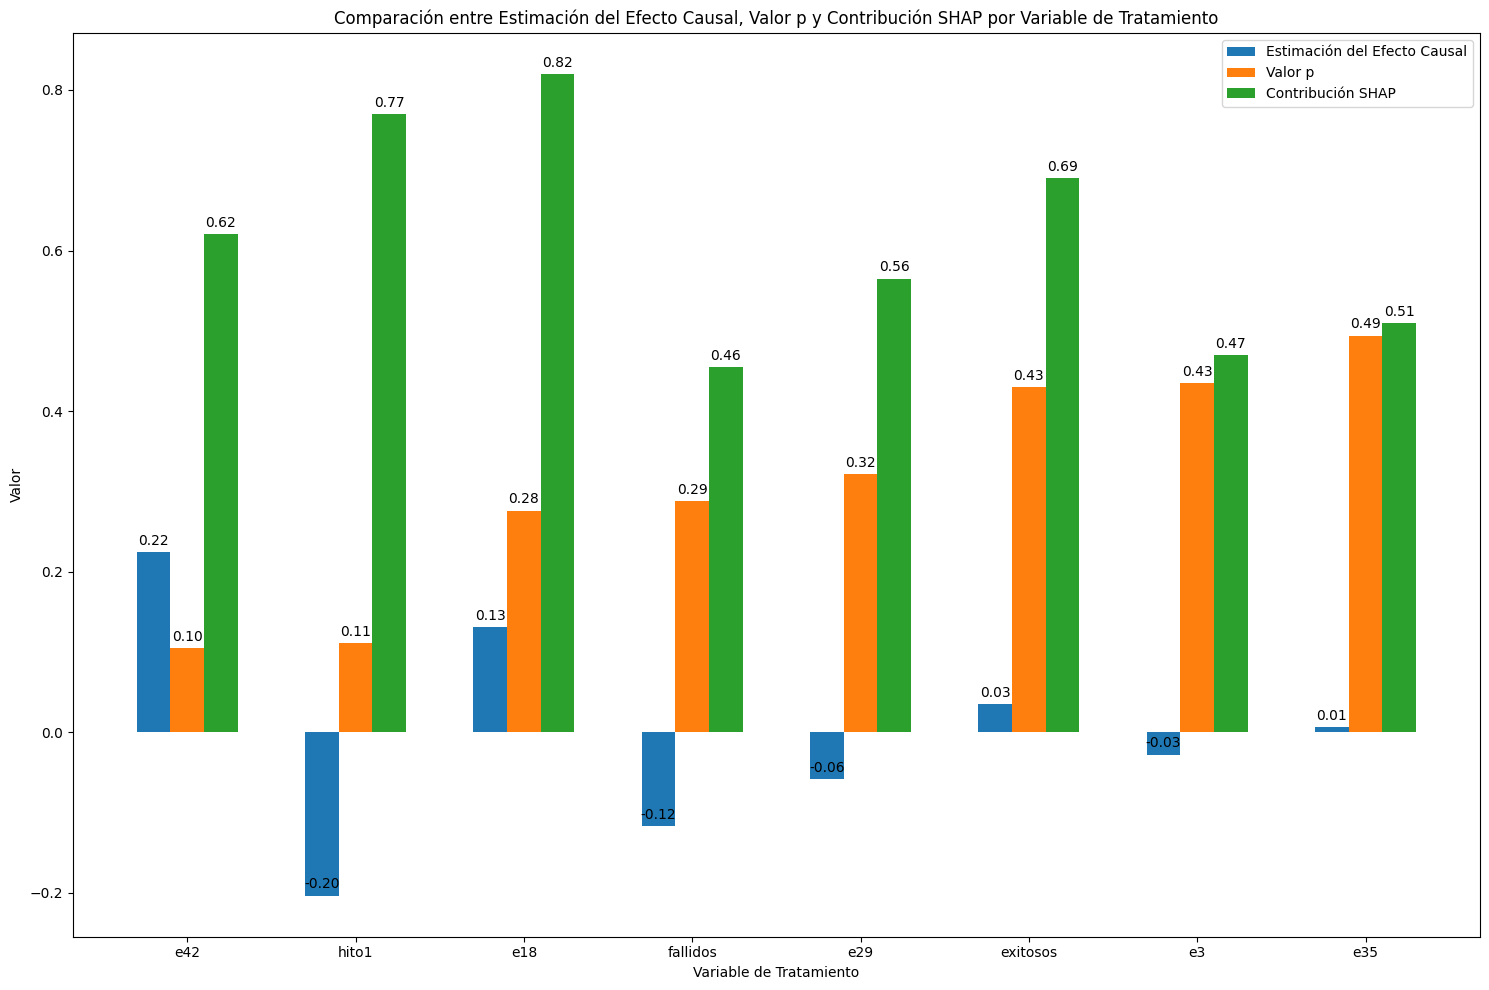
\includegraphics[width=0.8\textwidth]{img/causalidad/grafico_resultados_variables_compara_shap.png}
    \caption{Comparación entre Estimación del Efecto Causal, Valor \( p \) y Contribución SHAP por Variable de Tratamiento.}
    \label{fig:grafico_comparativo_dowhy_shap}
\end{figure}

Los datos utilizados para generar este gráfico fueron registrados manualmente según los resultados obtenidos en lo largo de esta investigación. A continuación, se presenta el código utilizado para crear el gráfico comparativo:

\begin{lstlisting}[language=Python, caption=Código para generar el gráfico comparativo, label=lst:codigo_grafico_comparativo]
# Creando un gráfico comparativo de los resultados
import pandas as pd
import matplotlib.pyplot as plt
import numpy as np

# Definiendo los datos
dfDS = pd.DataFrame(
    {
        "Variable de Tratamiento": [
            "hito1",
            "fallidos",
            "exitosos",
            "e42",
            "e35",
            "e29",
            "e18",
            "e3",
        ],
        "Estimación del Efecto Causal": [
            -0.203623,
            -0.117432,
            0.034945,
            0.224736,
            0.006278,
            -0.058810,
            0.130773,
            -0.027964,
        ],
        "Valor p": [0.111, 0.288, 0.430, 0.105, 0.494, 0.322, 0.276, 0.435],
        "Contribución SHAP": [
            0.77,
            0.455,
            0.69,
            0.62,
            0.51,
            0.565,
            0.82,
            0.47,
        ],  # Asumiendo estos como los valores promedio de SHAP
    }
)
# Ordenar el DataFrame por el valor p (de más relevante a menos relevante)
dfDS = dfDS.sort_values(by="Valor p", ascending=True)
x = np.arange(len(dfDS))  # las ubicaciones de las etiquetas
width = 0.2  # el ancho de las barras

# Creando el gráfico
fig, ax = plt.subplots(figsize=(15, 10))

# Definiendo las barras
rects1 = ax.bar(
    x - width,
    dfDS["Estimación del Efecto Causal"],
    width,
    label="Estimación del Efecto Causal",
)
rects2 = ax.bar(x, dfDS["Valor p"], width, label="Valor p")
rects3 = ax.bar(x + width, dfDS["Contribución SHAP"], width, label="Contribución SHAP")

# Agregar etiquetas, título y leyenda
ax.set_xlabel("Variable de Tratamiento")
ax.set_ylabel("Valor")
ax.set_title(
    "Comparación entre Estimación del Efecto Causal, Valor p y Contribución SHAP por Variable de Tratamiento"
)
ax.set_xticks(x)
ax.set_xticklabels(dfDS["Variable de Tratamiento"])
ax.legend()

# Función para autolabel
def autolabel(rects):
    for rect in rects:
        height = rect.get_height()
        ax.annotate(
            "{:.2f}".format(height),
            xy=(rect.get_x() + rect.get_width() / 2, height),
            xytext=(0, 3),  # 3 puntos de compensación vertical
            textcoords="offset points",
            ha="center",
            va="bottom",
        )

# Aplicando la función autolabel
autolabel(rects1)
autolabel(rects2)
autolabel(rects3)

# Ajustando el layout y mostrando el gráfico
fig.tight_layout()
plt.show()
\end{lstlisting}





\textbf{Resumen:}

El análisis se enfocó en expandir la exploración inicial realizada en la variable \texttt{hito1} a otras variables de interés identificadas en la predicción SHAP. Se estableció un proceso analítico iterativo, encapsulado en la función \texttt{run\_causal\_model}, que se ejecutó sobre cada variable en el array \texttt{preguntasGuia}. Se almacenaron los resultados en una lista \texttt{results} para un análisis posterior y comparación. A través de este proceso, se obtuvieron estimaciones del efecto causal y valores p para cada variable, que se detallaron en una tabla y se visualizaron en un gráfico. Además, se realizó una comparación entre los resultados obtenidos con SHAP y DoWhy, mostrando cómo estas dos metodologías proporcionan insights diferentes pero complementarios sobre la influencia de las variables en la probabilidad de aprobar la primera evaluación del curso.

\textbf{Conclusión Final:}

El ejercicio analítico realizado proporciona una visión integral y profunda sobre cómo ciertas variables, asociadas a una guía de apoyo, podrían afectar la probabilidad de aprobar la primera evaluación del curso. Se logró una comprensión inicial de la variable \texttt{hito1} y su relación con la variable de resultado \texttt{aprobado}, y se expandió este análisis a otras variables relevantes, utilizando un proceso iterativo que proporcionó estimaciones del efecto causal y evaluaciones de significancia estadística.

La comparativa entre los análisis de SHAP y DoWhy revela cómo diferentes perspectivas y metodologías pueden enriquecer la comprensión sobre las relaciones entre las variables y el rendimiento académico. Mientras SHAP proporciona una descomposición de la contribución de cada variable al modelo predictivo, DoWhy permite explorar la causalidad entre las variables.

Este trabajo destaca la importancia de evaluar las suposiciones del modelo y considerar variables confundidoras en la interpretación de los resultados. Además, subraya la relevancia de una validación cruzada y una visualización efectiva para una mejor comprensión y comunicación de los hallazgos.

En resumen, los insights obtenidos a través de este análisis ofrecen una base sólida para futuras investigaciones y pueden servir como guía para implementar estrategias de apoyo dirigidas a mejorar el rendimiento académico de los estudiantes. Sin embargo, es crucial tener en cuenta que la interpretación del impacto y relevancia de las variables requiere un examen cuidadoso de las suposiciones del modelo y, posiblemente, una exploración adicional a través de análisis de sensibilidad o recopilación de datos adicionales.


